
\section{funzioni trigonometriche, radianti}
%%%%%%%%%%%
%%%%%%%%%%%

Nel capitolo~\ref{sec:funzioni_trigonometriche} abbiamo definito le 
funzioni $\sin$ e $\cos\colon \RR\to \RR$ con periodo $\tau>0$ (arbitrario)
in modo tale che la funzione $\phi\colon \RR\to\RR^2$, $\phi(t)=(\cos t, \sin t)$ 
percorra, con moto circolare uniforme, in senso antiorario, la circonferenza 
unitaria $\ENCLOSE{(x,y)\in \RR^2\colon x^2+y^2=1}$.
Tale funzione descrive in effetti un moto circolare uniforme 
in quanto percorre archi congruenti in tempi uguali.
\mynote{Due figure geometriche sono \emph{congruenti} se c'è una isometria 
che manda una nell'altra.
Due archi sono congruenti se hanno la stessa lunghezza e lo stesso raggio, 
ma non è necessario introdurre il concetto di \emph{lunghezza d'arco} per parlare 
di congruenza.
}

Vogliamo ora mostrare che è possibile scegliere la costante $\tau$
in modo tale che la linea descritta da $\phi$ percorra la circonferenza 
con \emph{velocità} unitaria.
\mynote{Ricordiamo che $\tau$ è il periodo delle funzioni $\phi$,
$\cos$ e $\sin$}%
Se seguo il punto $f(t)$ a partire dall'istante $t=0$ per un breve tempo 
$\Delta t\neq 0$
osservo che il punto si sposta tra $f(0) = (1,0)$ e 
$f(\Delta t) = (\cos \Delta t, \sin \Delta t)$.
\mynote{La notazione $\Delta t$ indica un qualunque numero positivo.
Usiamo tale notazione perché tale numero rappresenta 
una differenza ($\Delta$ è una lettera $D$ greca)
di tempi tra loro vicini.}%
Intuitivamente quando $t=0$ il punto $f(t)$ si muove verticalmente, 
verso l'alto. 
Lo spazio percorso $\Delta s$ sarà quindi approssimativamente 
uguale alla variazione della coordinata $y$: 
$\Delta y = \sin \Delta t$.
\mynote{Ricordiamo che $\sin 0 = 0$}
Dunque la velocità sarà pari alla componente verticale della velocità 
e sarà, intuitivamente, il limite di $\frac{\Delta y}{\Delta t}$ ovvero 
\mynote{Vedremo tra poco che questo limite è la  
\emph{derivata} della funzione $f$ nel punto $t=0$.}
\[
\lim_{\Delta t\to 0} \frac{\sin(\Delta t)}{\Delta t}.  
\]

Dal punto di vista formale non è del tutto ovvio che questo limite esista.
Nel seguito lo dimostriamo, con un metodo molto simile a quello utilizzato 
per definire la costante $e$ di Nepero.
Così come l'esponenziale reale $x\mapsto a^x$ 
è un isomorfismo tra il gruppo additivo di $\RR$ e il gruppo moltiplicativo 
di $\RR^+$, così la funzione $\phi(t) = (\cos(t), \sin(t))$ 
risulta essere un isomorfismo 
tra il gruppo additivo $\RR$ e il gruppo delle rotazioni del piano che può essere 
rappresentato dall'insieme $U$ dei numeri complessi unitari.
Abbiamo già visto che affinché il punto che si muove con legge 
oraria $x\mapsto a^x$ abbia velocità $1$ per $x=0$ 
si deve porre $a=e$, la base dei logaritmi naturali.
Allo stesso modo vedremo ora che affinché la velocità 
del punto $t\mapsto \phi(t)$ 
sia anch'essa unitaria bisogna avere $\tau = 2\pi$.
Mettendo assieme i due isomorfismi $e^t$ e $\phi(t)$ si potrà definire,
come vedremo tra poco, un isomorfismo tra il gruppo additivo $\CC$ 
e il gruppo moltiplicativo $\CC\setminus\ENCLOSE 0$.
Quello che si ottiene è l'esponenziale complesso $z\mapsto e^z$. 
La velocità di $\phi(t)$ rappresenta in effetti la derivata di tale funzione 
complessa nel punto $1$ nella direzione dell'asse immaginario 
così come la derivata della funzione esponenziale reale è la derivata 
nella direzione reale. 
Si intuisce così come le costanti fondamentali $e$ e $\pi$ siano legate 
tra loro dalla condizione di fare sì che la funzione esponenziale complessa 
sia derivabile in senso complesso ed abbia derivata complessa pari a $1$.

\subsection{il numero $\pi$}

In questo capitolo dobbiamo lavorare con le funzioni 
$\sin$, $\cos$ e $\tg=\frac{\sin }{\cos}$ introdotte 
nel capitolo~\ref{sec:funzioni_trigonometriche}. 
Queste funzioni sono state definite con un periodo $\tau>0$
fissato in modo arbitrario a partire dalla funzione $\phi$ definita 
dal Teorema~\ref{th:omomorfismo_U}. 
Scriveremo $\phi_\tau$,
$\sin_\tau$ e $\cos_\tau$ quando è utile mettere in evidenza 
la dipendenza da $\tau$. 
In questo capitolo definiremo il numero $\pi$ e a quel 
punto si sceglierà sempre $\tau=2\pi$ come misura dell'angolo giro.

Se scegliamo due diverse misure $\tau$ e $\sigma$ per l'angolo giro, 
la relazione tra le due funzioni è semplicemente:
\begin{equation}\label{cambio_angolo}
  \phi_\tau (\tau t) = \phi_1(t) = \phi_\sigma(\sigma t), 
\end{equation}
in quanto $\phi_\tau(\tau t)$ soddisfa le proprietà che 
definiscono in modo univoco $\phi_1$ in base al Teorema~\ref{th:omomorfismo_U}.

\begin{theorem}
\label{teo_limite_pi}
Per ogni $x\in \RR$ con $0<x \le \frac \tau 2$, la successione
\[
    a_n = n \sin_\tau \frac x n
\]
converge ad un limite finito, positivo.
\end{theorem}
%
\begin{proof}
Faremo uso della funzione $\tg x= \frac{\sin x}{\cos x}$.
Useremo le formule di addizione:
\begin{align*}
 \sin(x+y) &= \sin x\cos y + \cos x \sin y,\\
 \cos(x+y) &= \cos x \cos y - \sin x \sin y  
\end{align*}
da cui, facendo il rapporto e dividendo numeratore 
e denominatore per $\cos x \cos y$ si ottiene:
\[
  \tg(x+y) = \frac{\tg x + \tg y}{1-\tg x \tg y}.
\]
Useremo anche il fatto che sull'intervallo 
$\closeinterval{0}{\frac \tau 4}$
\mynote{ricordiamo che $\tau$ è il periodo (scelto arbitrariamente)
delle funzioni $\sin$ e $\cos$} 
le funzioni $\sin$ e $\cos $
hanno valori compresi tra $0$ e $1$.
Queste proprietà sono garantite 
dal teorema~\ref{th:proprieta_trigonometriche}.
La funzione $\tg x$ a sua volta è definita se $0\le x < \frac \tau 4$
(visto che $\cos \frac \tau 4=$, la tangente non è definita per $x=\frac \tau 4$).

\emph{Passo 1:}
vogliamo dimostrare che se $n\in \NN$ e $t>0$, si ha
\begin{equation}\label{eq:4813509}
  nt <\frac \tau 4
  \implies
  n\sin t\le \tg nt.
\end{equation}
Lo dimostriamo per induzione.
Se $n=0$ è ovvio.
Supponendo \eqref{eq:4813509} vera per un certo $n$
vogliamo ora dimostrare che se $(n+1)t < \frac \tau 4$
si ha $(n+1)\sin t \le \tg (n+1)t$.
Osserviamo che se $(n+1)t<\frac \tau 4$ anche $nt < \frac \tau 4$ e 
le funzioni $\sin,\cos$ e $\tg$ sono tutte positive nei punti 
$t$, $nt$ e $(n+1)t$.
Dunque si ha:
\begin{align*}
\tg (n+1) t 
  &= \frac{\tg nt + \tg t}{1-\tg nt \tg t}
  \ge \tg nt + \tg t \\
  &\ge n\sin t + \tg t \qquad\text{[per \eqref{eq:4813509}]}\\
  &\ge n\sin t + \sin t
  =(n+1)\sin t. 
\end{align*}

\emph{Passo 2:}
dimostriamo che se $n\ge 2$ allora risulta $a_{n+1} \ge a_n$.
Per poter applicare \eqref{eq:4813509} 
ci serve avere $nt < \frac \tau 4$ cioè $\frac x {n+1}< \frac \tau 4$
che è vero essendo $x\le \frac \tau 2$ e $n\ge 2$.
Dunque, posto $t = \frac{x}{n(n+1)}$, si ha:
\begin{align*}
  a_n &= n \sin\frac{x}{n+1} 
    = n \sin (n+1)t
    = n \sin nt \cos t + n \sin t \cos nt\\
    &\le n \sin nt \cos t + \tg nt \cos nt
    \qquad\text{[per \eqref{eq:4813509}]}\\
    &\le n \sin nt + \sin nt
    = (n+1) \sin nt = (n+1) \sin \frac x n.
\end{align*}

\emph{Passo 3:}
la successione $a_{3n}$ è limitata.
Infatti si ha
\begin{align*}
 a_{3n} = 3n \sin \frac x {3n} 
 \le 3\tg \frac x 3
\end{align*}
dove abbiamo potuto applicare~\eqref{eq:4813509}
visto che $\frac x 3 < \frac{\tau }{2}$
essendo $x\le \frac {\tau} 2$.

\emph{Passo 4: conclusione.}
Per il passo 2 la successione $a_{n+1}$ è crescente,
dunque per il Teorema~\ref{th:limite_successione_monotona} la successione 
ha limite $a_n\to \ell$ per $n\to +\infty$.
Visto che $a_n \ge a_2$ per ogni $n\ge 2$ si ha $\ell \ge a_2 >0$.
E, per il passo 3, non può essere $\ell=+\infty$ altrimenti $a_{3n}$ 
non sarebbe limitata.
\end{proof}

Diamo una interpretazione geometrica del risultato precedente.
Vogliamo calcolare la lunghezza di un arco di misura $x$
sulla circonferenza unitaria. 
Dividiamo l'arco in $n$ parti uguali e consideriamo 
la poligonale formata dalle corde sugli $n$ angoli di misura 
$\frac {x} n$. 
In generale la corda sull'angolo $\alpha$ di una circonferenza 
di raggio $r$ misura $2r \sin \frac \alpha 2$.
Dunque la poligonale costruita sull'arco $x$ 
misura $n\sin\frac{x}{2n}$.
Vorremmo quindi definire $\pi$ come il limite di questa successione.

\begin{definition}[$\pi$ costante fondamentale della trigonometria]%
  \label{def:pi}%
Definiamo
\[
 \pi 
  \defeq \lim_{n\to +\infty} n\cdot \sin_\tau \frac \tau {2n}.
\]
dove $\sin_\tau$ è la funzione $\sin$ costruita nel 
teorema~\ref{def:sin_cos} con periodo $\tau$.
Visto che $\sin_\tau \tau x = \sin_\sigma \sigma x$ il limite 
non dipende dalla scelta di $\tau$.
Questo limite esiste ed è finito e positivo per il Teorema~\ref{teo_limite_pi}.
\end{definition}

Scegliendo $\tau = 360$ si trova $a_4 = 4 \sin_\tau \frac{180}{4} = 2 \sqrt 2 > 2.8$ da cui,
per la proprietà di monotonia di $a_n$, si trova $\pi > 2.8$.
Osservando che $a_{2^n} = 2^n \sin_\tau \frac{45}{2^{n-2}}\le 4 \tg_\tau 45 = 4$
si ottiene $\pi<4$.
Troveremo dei metodi molto più raffinati per determinare i valori approssimati 
di $\pi$, si veda ad esempio l'esercizio~\ref{ex:cifre_pi} e la 
tabella~\ref{tab:cifre_pi}.

\begin{theorem}[limite notevole $\sin$]
  \label{th:limite_notevole_sin}%
Per ogni $x\in\RR$, $x\neq 0$ si ha 
\[
\lim_{x\to 0}\frac{\sin_{\tau} x}{x}
= \frac{2\pi}{\tau}.
\]
In particolare se scegliamo $\tau = 2\pi$ si ha
il limite notevole:
\begin{equation}\label{eq:limite_notevole_sin}
 \lim_{x\to 0} \frac{\sin x}{x} = 1.
\end{equation}
\end{theorem}
%
\begin{proof}
Mostriamo innanzitutto che si ha
\begin{equation}\label{eq:771743}
   \lim_{t\to+\infty} t \sin_\tau \frac{\tau}{2t} = \pi.
\end{equation}
Infatti 
\begin{equation}\label{eq:4961077}
  \frac{\lfloor t \rfloor}{\lceil t \rceil} \cdot \lceil t \rceil \sin_\tau \frac{\tau}{2\lceil t \rceil}
  \le \lfloor t \rfloor \sin_\tau \frac{\tau}{2\lceil t \rceil}
  \le t \sin_\tau \frac{\tau}{2t} 
  \le \lceil t \rceil \sin_\tau \frac{\tau}{2\lfloor t \rfloor}
  \le \frac{\lceil t \rceil}{\lfloor t \rfloor} \cdot \lfloor t \rfloor \sin_\tau \frac{\tau}{2\lfloor t \rfloor}
\end{equation}
e visto che 
\[
  \frac{\lfloor t \rfloor}{\lceil t \rceil}\to 1, \qquad
  \frac{\lceil t \rceil}{\lfloor t \rfloor}\to 1
\]
per la definizione di $\pi$, entrambi gli estremi della catena 
di disuguaglianze~\eqref{eq:4961077} tendono a $\pi$
e dunque per il teorema dei carabinieri
si ottiene il limite volute~\eqref{eq:771743}.
Con il cambio di variabile $x=\frac 1 t$ si ottiene 
il limite~\eqref{eq:limite_notevole_sin} quando $x\to 0^+$.
Il limite completo per $x\to 0$ si ottiene per simmetria.
\end{proof}

D'ora in avanti sceglieremo $\tau=2\pi$ come periodo 
delle funzioni trigonometriche.
E d'ora in avanti si intenderà $\sin = \sin_{2\pi}$, 
$\cos = \cos_{2\pi}$. Si avrà quindi il limite notevole 
\[
   \lim_{x\to 0} \frac{\sin x}{x} = 1.  
\]

Quando introdurremo le derivate potremo anche osservare che 
questa scelta del periodo $\tau=2\pi$ 
fa sì che il punto di coordinate
$(\cos t,\sin t)$ si muova con velocità unitaria lungo 
la circonferenza unitaria. 
Dunque tale punto percorre un arco di lunghezza $t$ nel tempo $t$.
In particolare in un periodo $\tau=2\pi$ il punto percorre l'intera 
circonferenza e dunque risulta che $2\pi$ è la lunghezza 
della circonferenza unitaria (ovvero $2\pi r$ è la lunghezza della circonferenza 
di raggio $r$).
Al tempo $t=1$ il punto $(\cos t,\sin t)$ individua un angolo che 
viene chiamato \emph{radiante} in quanto corrisponde ad un arco di lunghezza 
pari al raggio (unitario). 
Dunque il \emph{radiante} è l'unità di misura naturale per misurare gli angoli 
e le funzioni $\sin$ e $\cos$ d'ora in poi saranno fissate con tale unità di misura.

\newsavebox{\qrfigtrigo}\sbox{\qrfigtrigo}{\myurlhere{figtrigo}{funzioni trigonometriche}}%
\begin{figure}
  \centering%
  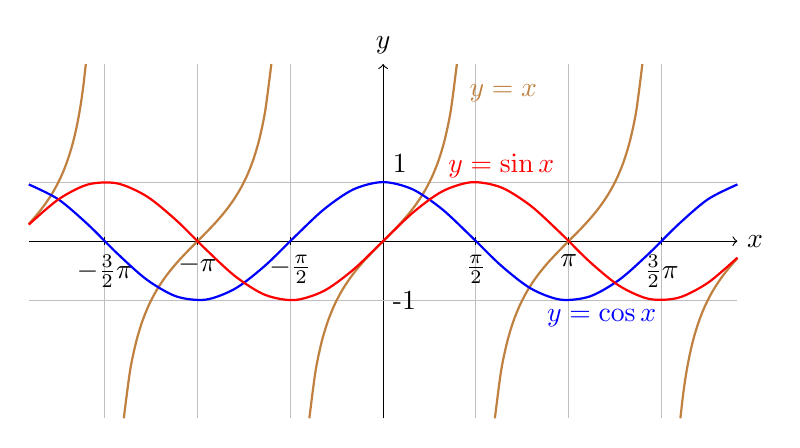
\begin{tikzpicture}[scale=0.75]
  \draw[->] (-6,0) -- (6,0) node[right] {$x$};
  \draw[->] (0,-3) -- (0,3) node[above] {$y$};
  \foreach \x/\xtext in
    {{pi/2}/{\frac \pi 2}, {pi}/{\pi}, {3*pi/2}/{\frac{3}{2}\pi},
    {-pi/2}/{-\frac \pi 2}, {-pi}/{-\pi}, {-3*pi/2}/{-\frac{3}{2}\pi}} {
    \draw[shift={(\x,0)},lightgray] (0,-3) -- (0,3);
    \draw[shift={(\x,0)}] (0pt,2pt) -- (0pt,-2pt) node[below] {$\xtext$};
  }
  \foreach \y in {1, -1} {
    \draw[shift={(0,\y)},lightgray] (-6,0) -- (6,0);
  }
  \draw (0,1) node [above right] {1};
  \draw (0,-1) node [right] {-1};
  \draw[domain=-rad(atan(3)):rad(atan(3)),smooth,variable=\x,brown,thick] plot ({\x},{tan(deg(\x))});
  \draw[domain=pi-rad(atan(3)):pi+rad(atan(3)),smooth,variable=\x,brown,thick] plot ({\x},{tan(deg(\x))});
  \draw[domain=-pi-rad(atan(3)):-pi+rad(atan(3)),smooth,variable=\x,brown,thick] plot ({\x},{tan(deg(\x))});
  \draw[domain=-6:-2*pi+rad(atan(3)),smooth,variable=\x,brown,thick] plot ({\x},{tan(deg(\x))});
  \draw[domain=2*pi-rad(atan(3)):6,smooth,variable=\x,brown,thick] plot ({\x},{tan(deg(\x))});
  \draw[domain=-6:6,smooth,variable=\x,blue,thick] plot ({\x},{cos(deg(\x))});
  \draw[domain=-6:6,smooth,variable=\x,red,thick] plot ({\x},{sin(deg(\x))});
  \draw (3.7,-1) node[blue,below] {$y=\cos x$};
  \draw (2,0.9)  node[red,above] {$y=\sin x$};
  \draw (1.3,2.5) node[brown,right] {$y=\tg x$};
  \end{tikzpicture}
  \caption{%
  I grafici delle funzioni $\sin$, $\cos$ e $\tg$.
  \ifwidemargin\\\\\fi%
  \usebox{\qrfigtrigo}}
\end{figure}

\subsection{funzioni trigonometriche inverse}

La funzione $\sin\colon[-\pi/2,\pi/2]\to [-1,1]$ 
risulta essere strettamente crescente e bigettiva. 
Dunque restringendo il dominio all'intervallo $[-\pi/2, \pi/2]$
e il codominio all'intervallo $[-1,1]$ la funzione risulta invertibile.
La funzione inversa
\[
  \arcsin\colon[-1,1]\to [-\pi/2, \pi/2]
\]
si chiama \emph{arco seno}. 
E' una funzione continua per il Teorema~\ref{th:monotona_continua}
di continuità delle funzioni monotòne.

Per definizione di funzione inversa si ha
\[
  \arcsin(\sin x) = x, \qquad \forall x \in [-\pi/2, \pi/2]
\]
e
\[
  \sin(\arcsin x) = x, \qquad \forall x \in [-1, 1].
\]

La funzione $\cos \colon[0,\pi] \to [-1,1]$ risulta essere strettamente
decrescente e bigettiva.
La funzione inversa
\[
  \arccos\colon[-1,1] \to [0,\pi]
\]
si chiama \emph{arco coseno}. 
Anch'essa è continua per le proprietà di monotonia.
Per definizione si ha
\[
  \arccos(\cos x) = x, \qquad \forall x \in [0,\pi]
\]
e
\[
    \cos(\arccos x) = x, \qquad \forall x \in [-1,1].
\]

La funzione
\index{tangente!funzione trigonometrica}
\mymargin{$\tg x$}%
\index{$\tg x$}
\[
\tg x = \frac{\sin x}{\cos x}
\]
è definita quando $\cos x\neq 0$ ovvero:
\[
  \tg \colon \RR \setminus\ENCLOSE{\frac \pi 2+ k\pi\colon k\in \ZZ} \to \RR.
\]
Se restringiamo la funzione all'intervallo $\enclose{-\pi/2, \pi/2}$ possiamo
facilmente osservare che la funzione $\tg\colon(-\pi/2,\pi/2)\to \RR$ è strettamente crescente. Inoltre se $a_n \to \pi/2$, $a_n<\pi/2$ si ha $\cos(a_n)\to 0$ (per continuità del coseno) e $\sin(a_n)\to 1$ dunque $\tg a_n\to +\infty$. Analogamente per $a_n \to -\pi/2$ si trova $\tg a_n \to -\infty$. Dunque per il teorema dei valori intermedi possiamo affermare che la funzione $\tg\colon(-\pi/2,\pi/2)\to \RR$ è suriettiva. E' quindi invertibile
e la funzione inversa
\[
  \arctg \colon \RR \to (-\pi/2,\pi/2)
\]
si chiama \emph{arco tangente}. Per definizione si ha
\[
  \arctg \tg x = x, \qquad \forall x \in (-\pi/2, \pi/2)
\]
e
\[
  \tg\arctg x = x, \qquad \forall x \in \RR.
\]

Grazie al teorema~\ref{th:monotona_continua}
visto che queste funzioni sono monotone e bigettive
possiamo affermare che
le funzioni $\arcsin$, $\arccos$ e $\arctg$ 
sono tutte funzioni continue.

\begin{exercise}[funzioni misteriose]
  Si disegni il grafico delle seguenti funzioni
  \[
    f(x) = \arcsin \sin x, \qquad 
    g(x) = \arccos \cos x, \qquad 
    h(x) = \arctg \tg x.
  \]
  Si osservi che:
  \begin{enumerate} 
    \item $f$ e $g$ sono definite su tutto $\RR$,
  mentre $h$ è definita su $\RR\setminus\ENCLOSE{\frac{\pi}2+k\pi\colon k\in \ZZ}$;
    \item $f$ e $h$ hanno valori 
  in $\closeinterval{-\frac \pi 2}{\frac \pi 2}$
  mentre $g$ ha valori in $\closeinterval{0}{\pi}$;
    \item $f$ e $g$ hanno periodo $2\pi$,
  $h$ ha periodo $\pi$;
    \item tutte e tre sono funzioni continue (sul loro dominio).
  \end{enumerate}
\end{exercise}

\begin{exercise}
Dimostrare che per ogni $x>0$ si ha
\[
  \arctg \frac 1 x = \frac \pi 2 - \arctg x.
\]
\end{exercise}

\begin{exercise}[lunghezza della circonferenza]
Si osservi che un $n$-agono regolare iscritto a una circonferenza 
di raggio $r$ ha lati di lunghezza $l_n = 2r\sin \frac{\pi}{n}$
e quindi perimetro $p_n = n\cdot l_n$.
Si verifichi che 
\[
  \lim_{n\to +\infty} p_n = 2\pi r.
\]
\end{exercise}
